%!TEX root = ../thesis.tex
%*******************************************************************************
%*********************************** First Chapter *****************************
%*******************************************************************************

\chapter{Introduction and motivation}  %Title of the First Chapter
\label{ch1}

\ifpdf
    \graphicspath{{Chapter1/Figs/Raster/}{Chapter1/Figs/PDF/}{Chapter1/Figs/}}
\else
    \graphicspath{{Chapter1/Figs/Vector/}{Chapter1/Figs/}}
\fi


%********************************** %First Section  **************************************

This doctoral dissertation includes two journal articles in preparation. This introduction overviews the overarching research motivation, key concepts, and research questions examined in each subsequent chapter. Each results chapter includes a detailed and specific introduction to the relevant research question.

\section{Motivation}


Aerosols refer to tiny particles suspended in the air, including dust, pollutants, and natural substances such as sea salt and pollen. They play an important role in the atmosphere as they moderate the Earth's radiation budget of the atmosphere through scattering and absorption of solar radiation \citep{szopaShortlivedClimateForcers2021}.  They serve as the nucleating particles for cloud formation, and their properties modulate cloud properties such as brightness, reflectivity and lifetime \citep{boucherCloudsAerosols2014}.  Aerosols also provide a medium for chemical reactions, enabling important heterogeneous chemical pathways \citep{seinfeldAtmosphericChemistryPhysics2016}.

Aerosols have a wide range of compositions and span a range from a few nanometres to tens of microns.  Their atmospheric lifetime ranges from minutes to weeks, sufficient for long-range transport across the globe \citep{liScatteringAbsorbingAerosols2022}.  

Tropospheric aerosol is dominated, by mass, by sea salt and mineral dust aerosol \citep{szopaShortlivedClimateForcers2021}.  In terms of radiation and particle number, other important classes are secondary aerosols such as sulfate, nitrate and biogenic aerosol \citep{liScatteringAbsorbingAerosols2022}. These are formed in the atmosphere via gas-particle conversion.  Soot forms the remaining broad class.  Mixtures of these compounds are commonly found throughout the atmosphere \citep[e.g.][]{jimenezEvolutionOrganicAerosols2009, bauerTurningPointAerosol2022}.

The atmospheric aerosol can be divided into broad classes according to size: the nucleation mode, around 10 nm, and Aitken mode particles, having radii less than 100 nm, are formed in the early stages of gas-particle transfer, and have a short lifetime controlled by loss via diffusion to existing particle surfaces; accumulation mode particles, 100 nm in size and larger, are formed by coalescence of smaller particles and condensational growth, diffuse more slowly and have a longer lifetime; finally, coarse-mode particles, which are usually formed through mechanical processes such as wave-breaking or re-suspension of solid particles such as sand or soil, have a short lifetime due to gravitational settling \citep{seinfeldAtmosphericChemistryPhysics2016}.

This thesis focuses on sulfate aerosol, which is formed from the oxidation of sulfur dioxide (\ce{SO2}), and which is a major source of cloud condensation nuclei \citep{boucherCloudsAerosols2014}. To assess the effects of sulfate aerosol effects on climate, global climate model development has been one of the central methods. The results from the first sulfur aerosol global circulation model to consider a full annual cycle of sulfur were published in 1991 and effort in this field has continued ever since, with most modern global climate models considering the sulfur cycle at some level of detail \citep{langnerGlobalThreedimensionalModel1991, liAssessmentCoupledModel2021}. As the number and complexity of climate models have grown, there have been attempts to inter-compare these models, such as AeroCom. The most recent intercomparison are RFMIP, PDRMIP and AerChemMIP, which formed part of the sixth phase of the Coupled Model Intercomparison Project (CMIP6) and features state-of-the-science models \citep[e.g.][]{eyringOverviewCoupledModel2016, collinsAerChemMIPQuantifyingEffects2017, gillettDetectionAttributionModel2016}. 

Early CMIP6 results indicated that, despite participating models' increasing sophistication, they did not all perform well in predicting surface temperature, with the period between 1950--1990 showing low bias with respect to observations, i.e. the models consistently underpredict surface temperature \citep{flynnClimateSensitivityHistorical2020, zhangRoleAnthropogenicAerosols2021}. This anomalous cooling was shown to be related to the aerosol amount in the atmosphere \citep{zhangRoleAnthropogenicAerosols2021}. Attributing the causes of this bias was made more complicated by the fact that \ce{SO2} emission varies over the historical period, affecting both local aerosol loading, i.e. direct scattering, and aerosol effects on the atmosphere, e.g. cloud albedo.

This dissertation aims to further investigate the sulfur budget in a CMIP6 model, the UKESM1, and attributes aerosol budget changes to different oxidants with a view to understanding quantitatively the drivers of sulfate loading as a preliminary step to understanding the causes of the low bias of CMIP6 models at a time when sulfur emissions were increasing rapidly. 


\section{Aerosol and Climate} %Section - 1.1 

Aerosols affect the Earth’s energy budget in a variety of ways, both directly via scattering or absorption, and indirectly via their effect on important terms in the energy budget, such as latent heat release or evapotranspiration and enhancing cloud formation and by modulating the cloud properties \citep{readGlobalEnergyBudgets2016}.  Other aerosol processes and properties are important: aerosols can absorb radiation, increasing the strength of the greenhouse effect; hygroscopicity governs cloud formation, and hence indirect effects and latent heat release. Figure \ref{fig:trenberth} shows the Earth's energy balance with the incoming solar radiation in blue arrows and outgoing Earth radiation in red \citep{kiehlEarthAnnualGlobal1997}.  It can be seen that many of these processes can be modified by changes to aerosol loading or their properties. 

\begin{figure}
    \centering
    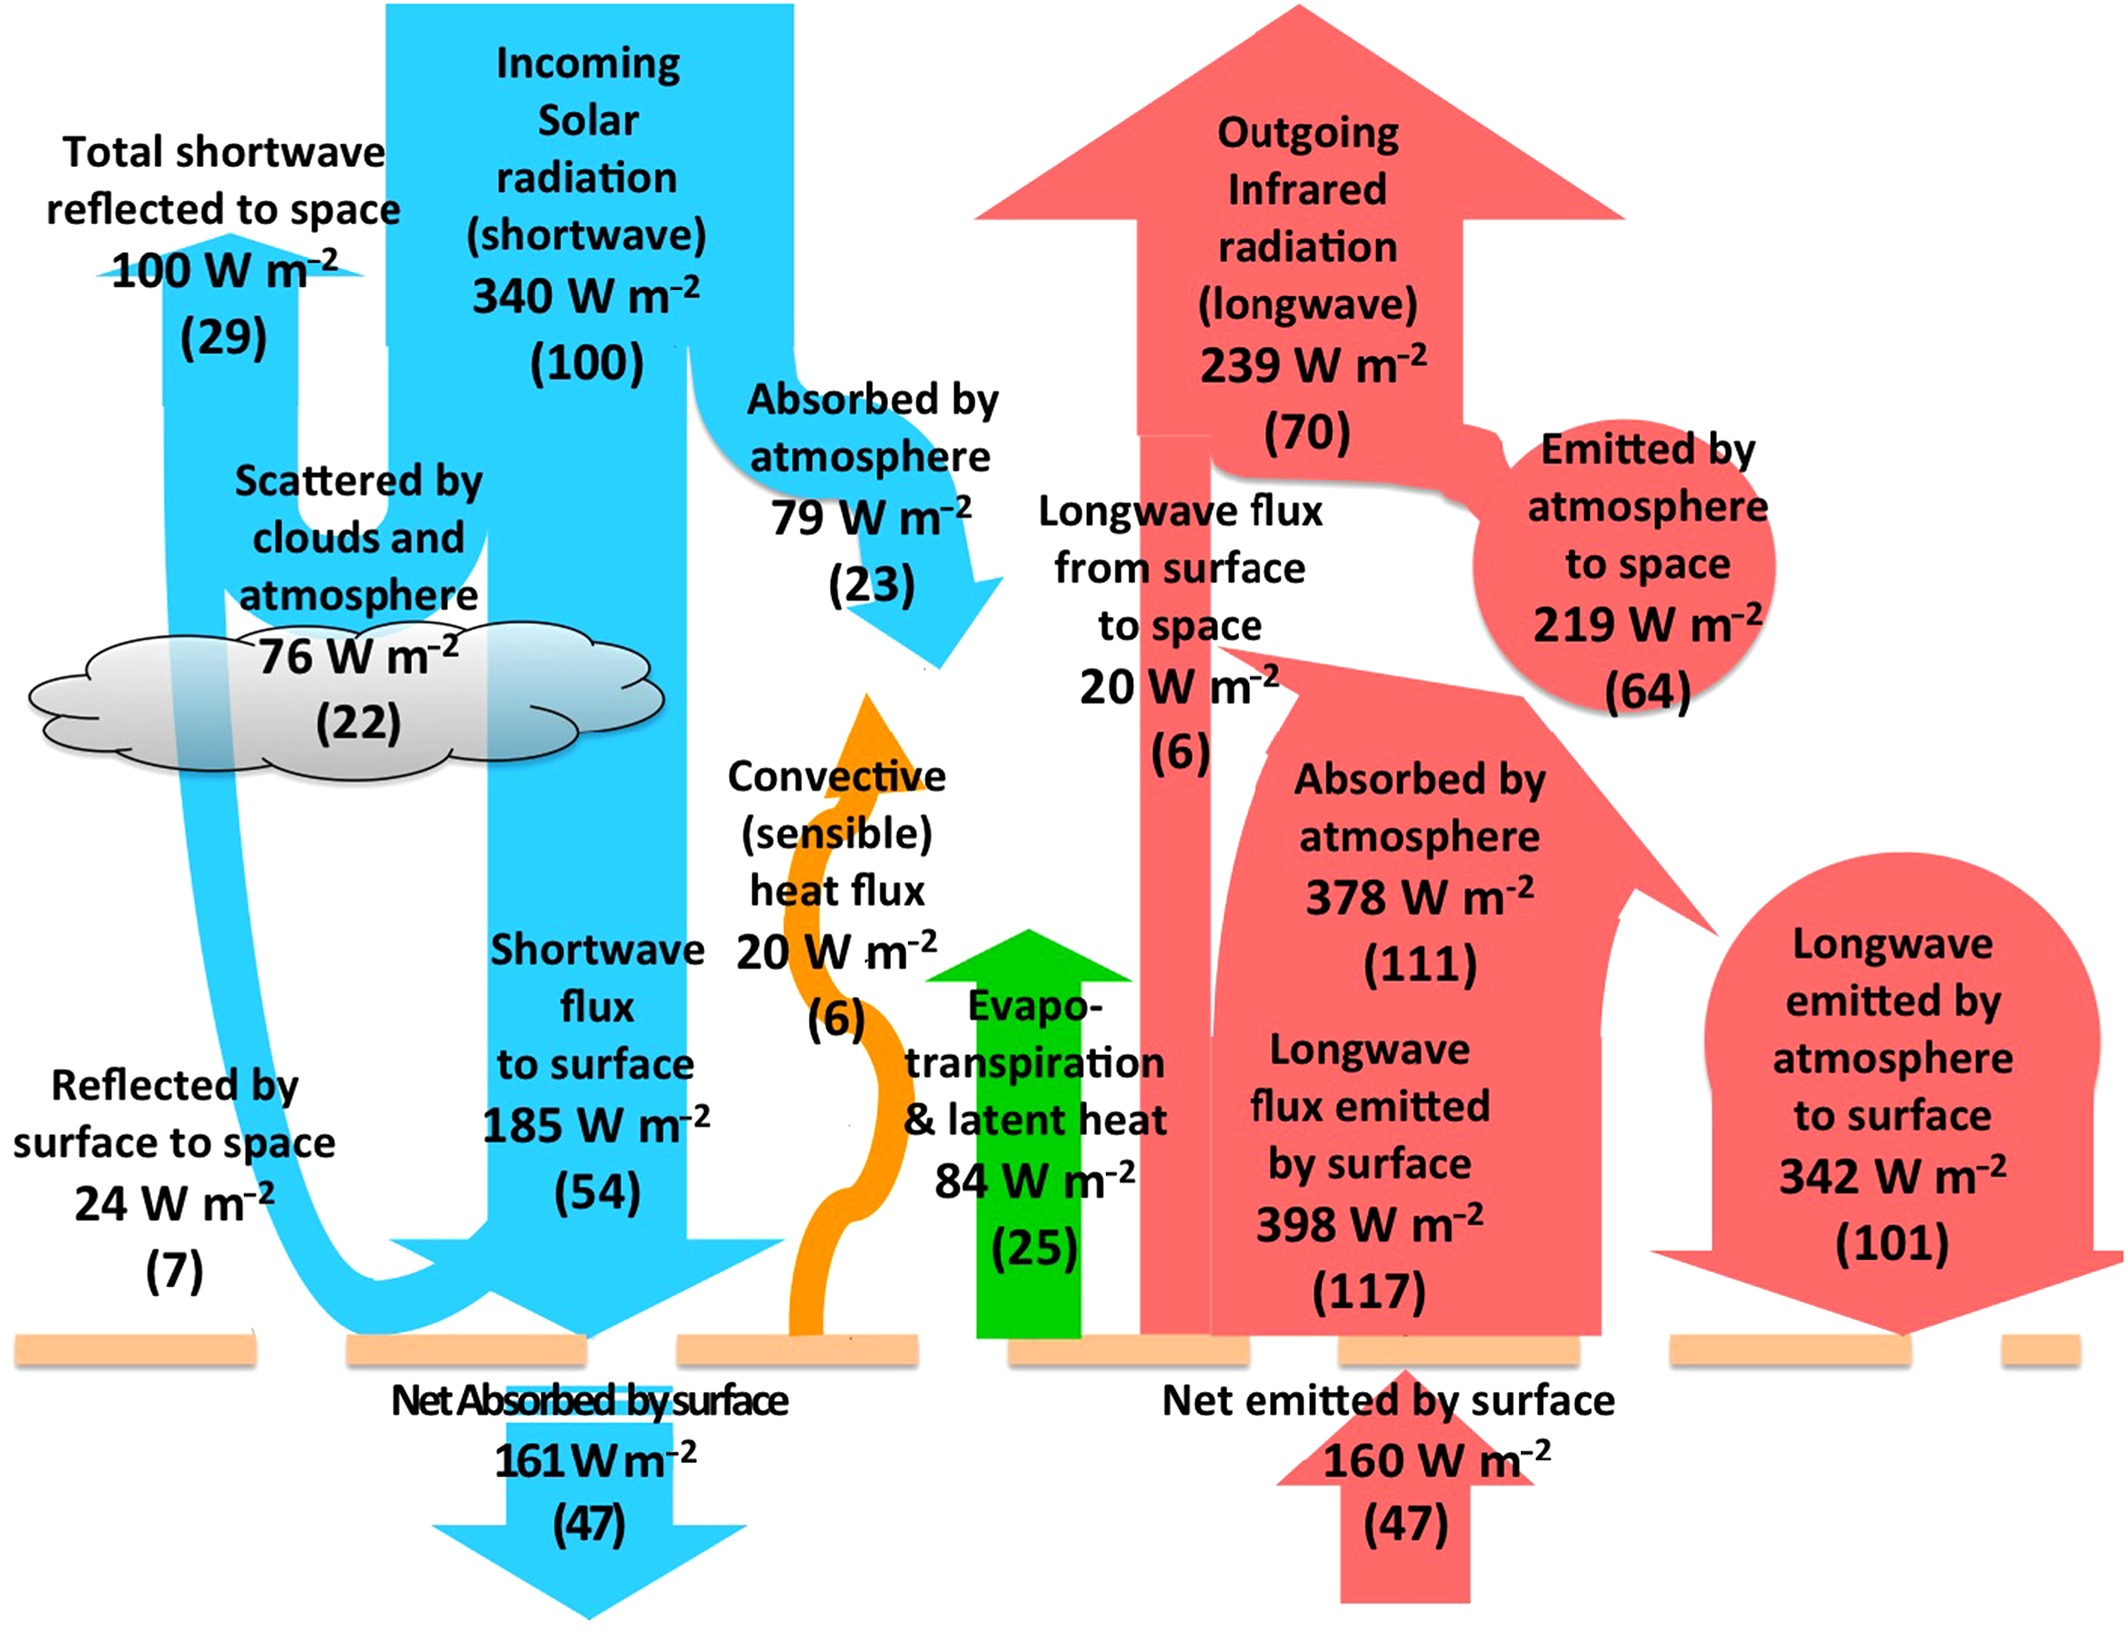
\includegraphics[width=0.7\columnwidth]{Chapter1/figs/01_trenberth.jpg}
    \caption[The Earth’s energy budget]{The Earth’s energy budget from \citet{readGlobalEnergyBudgets2016}, first used in \citet{kiehlEarthAnnualGlobal1997}}
    \label{fig:trenberth}
\end{figure}


There are many physical processes that affect the Earth's energy budget, with impacts at different times and spatial scales, such as increased carbon dioxide concentration and surface albedo change \citep{forsterEarthEnergyBudget2021}. A consistent way to characterize the behaviour of the climate system is therefore needed, ideally by using global-scale metrics on a common scale. One such metric is radiative forcing.

\subsection{Concept of radiative forcing}

Radiative forcing is a concept for quantifying the effects of physical processes that perturb the Earth's energy budget, connecting the effect of each individual perturbation to radiation changes and hence to global surface temperature response \citep{thornhillEffectiveRadiativeForcing2021}. The most recent IPCC report employs the definition of Effective Radiative Forcing (ERF) as the principal metric for quantifying such physical perturbations \citep{forsterEarthEnergyBudget2021}. 

In short, the global surface air temperature (GSAT) responds to a perturbation from a certain radiative forcing that gives rise to an energy imbalance at the top of atmosphere (TOA). This could be written as the linear energy budget equation.

\begin{equation}
\label{eq:erf}
    \Delta N = \Delta F - \alpha \Delta T
\end{equation}

Here, $\Delta N$ (W m$^{-2}$) denotes the change in the top-of-atmosphere net downward radiative flux, which is the result of the effective radiative forcing perturbation $\Delta F$ (W m$^{-2}$). $\alpha$ is the net feedback parameter and $\Delta T$ ($^\circ$C) is the change in global surface air temperature. 

Figure \ref{fig:1.ERF} shows the pre-industrial to present-day effective radiative forcing estimates for 1750 to 2019 for the concentration change in different forcing agents as featured in the Intergovernmental Panel on Climate Change (IPCC) assessment report (AR) 6 \citep{forsterEarthEnergyBudget2021}. Carbon dioxide (\ce{CO2}), ozone (\ce{O3}) and other well-mixed gases have positive radiative forcing, which means they exert a warming effect on global surface air temperature. In contrast, both aerosol-cloud and aerosol-radiation ERFs are negative. Moreover, aerosol effective radiative forcing also has the largest uncertainty of all forcings assessed in the IPCC report.

\begin{figure}
    \centering
    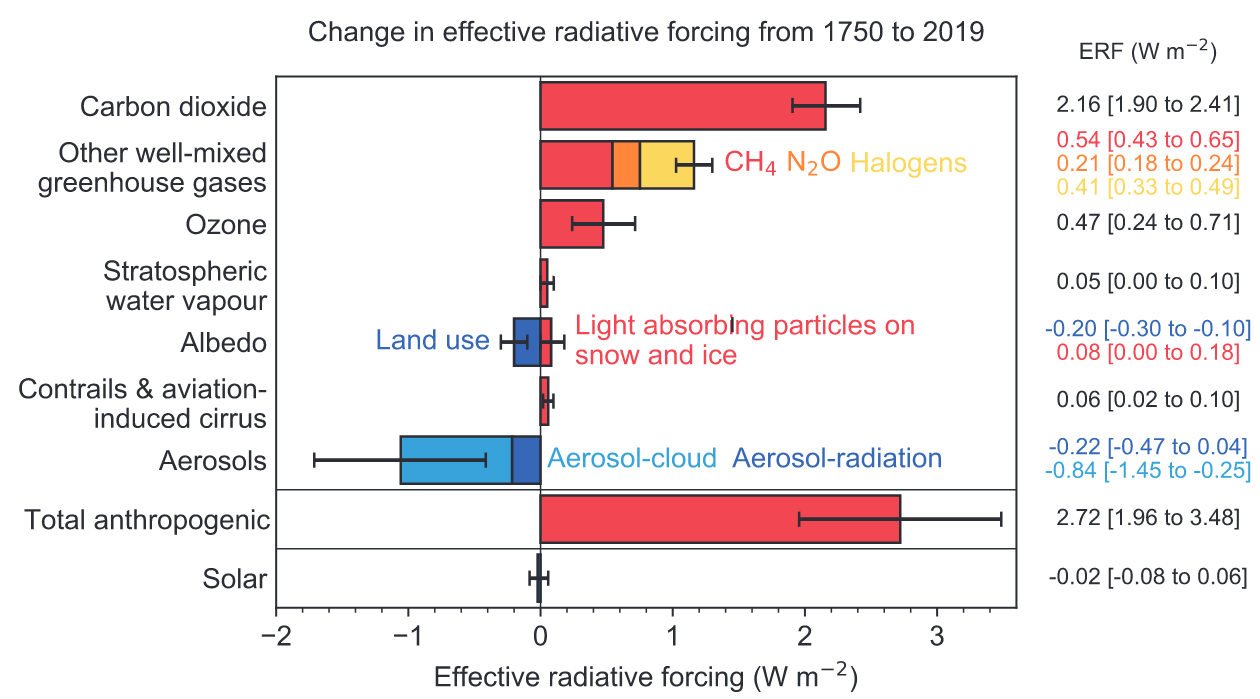
\includegraphics[width=6in]{Chapter1/figs/02_ERF.png}
    \caption[Effective radiative forcing (ERF) from 1750 to 2019]{Change in effective radiative forcing (ERF) from 1750 to 2019 by contributing forcing agents. Solid bars error bars represent best estimates and 5-95\% ranges. Figure from \citet{forsterEarthEnergyBudget2021}.}
    \label{fig:1.ERF}
\end{figure}

There are two approaches to evaluating ERF using climate simulations \citep[e.g.][]{gregoryNewMethodDiagnosing2004, oconnorAssessmentPreindustrialPresentday2021}.  The first method is to apply a step change to the forcing. This will immediately cause energy imbalance which will decrease as the system readjust itself back to the equilibrium ($\Delta N=0$). Equation \ref{eq:erf} gives the linear relationship between the annual global average temperature change to the annual energy imbalance. The linear relationship is assumed and the y-intercept is the value of ERF. This is usually referred to as the Gregory or the regression-based method \citep{gregoryNewMethodDiagnosing2004}. Another method is to set the $\Delta T$ term to zero. However, it is difficult to do so, so most studies prescribe sea surface temperature (SST) and sea ice concentration. A pair of simulations with and without the change in forcing is then performed for the fixed SST (fSST) simulations to estimate ERF as the difference in TOA radiative flux \citep{myhreNewEstimatesRadiative1998}. 


Effective radiative forcing is a good predictor of climate because the ratios of surface temperature change to forcing resulting from perturbations of different forcings are comparable \citep{myhreAnthropogenicNaturalRadiative2013, boucherCloudsAerosols2014}. One of the collaborative efforts to estimate effective radiative forcing from models is the CMIP which is detailed in section \ref{sec:1.CMIP6}


\subsection{Role of aerosol on climate}

The effective radiative forcing due to aerosols can be divided into aerosol-radiation interaction (ERFari) and aerosol-cloud interaction \citep[ERFaci;][]{ghanTechnicalNoteEstimating2013}. The aerosol direct effect, also referred to as aerosol-radiation interaction, can be observed locally e.g. from above the aerosol layer, such as from an aeroplane or from a mountaintop, as the layer scatters light, causing the appearance of a white or light-coloured hazy layer \citep{twomeyInfluencePollutionShortwave1977}. Such processes reduce solar radiation that reaches the Earth’s surface, with the optical depth depending on the total column mass burden of aerosol particles, but also on the size distribution and the particles’ optical properties. Not all types of aerosols scatter radiation with the same efficiency and some aerosols, such as soot, can also absorb solar radiation, as manifested in their naturally darker colour. 

The aerosol indirect effect, or aerosol-cloud interaction, encompasses the effects of aerosols on clouds and can be further divided into the effects of aerosol on cloud amount, cloud lifetime and cloud albedo.  Aerosols serve as cloud condensation nuclei and promote cloud formation \citep{albrechtAerosolsCloudMicrophysics1989}.  Changes in aerosol concentration are connected to variations in the cloud droplet size and number distribution. When there are more aerosols, cloud droplets are smaller. These clouds have less water content and appear brighter white, and, as a consequence, reflect more sunlight back to space, increasing planetary albedo. Examples of observed aerosol effects on the Earth’s atmosphere include volcanic aerosols \citep[e.g.][]{malavelleStrongConstraintsAerosol2017}, such as the 1991 eruption of Mount Pinatubo \citep{hansenPotentialClimateImpact1992}, and aerosols from ship tracks \citep{twohyEvaluationAerosolIndirect2005}. 



\section{Climate change and trends in short-lived climate forcers emissions and concentration}

% General idea of gases and pollutants that increase since PI
Anthropogenic emissions have generally increased since 1850 due to the accelerated industrialisation of the economy. This has led to an x-fold increase in methane emissions, an x-fold increase in CO2 both of which are greenhouse gases. 

% Specific increases of CH4 
Specific increases of CH4 

% idea of atmospheric oxidative power
idea of atmospheric oxidative power

% Changes to oxidants such as O3 and OH
Changes to oxidants such as O3 and OH

\section{Global tropospheric sulfur and sulfate aerosol budget}

Sulfate aerosol is emitted from both anthropogenic and natural sources, and is also produced from chemical production in the atmosphere by gas or aqueous phase reactions of sulfur dioxide (\ce{SO2}), dimethyl sulfide (DMS) and carbonyl sulfide \citep[OCS;][]{belvisoAssessmentMarineBiota2000}. After \ce{SO2} is released into the troposphere, it oxidises and forms sulfate aerosol.  The tropospheric sulfur cycle is closed by wet and dry deposition.

\begin{figure}
    \centering
    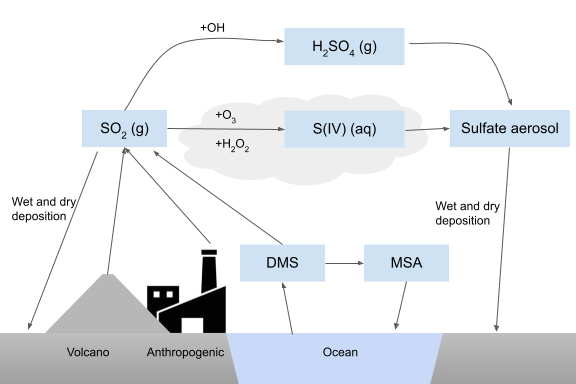
\includegraphics[width=6in]{Chapter1/figs/sulfur_budget.png}
    \caption[Summary of atmospheric sulfur budget]{Summary of atmospheric sulfur budget}
    \label{fig:sulfur-budget}
\end{figure}

\subsection{\ce{SO2} primary emission}

Primary emission of \ce{SO2} from natural sources comes from volcanic activities. Both continuously degassing volcanoes and sporadic eruptive volcanoes contribute to the Earth's tropospheric \ce{SO2} amount. Together, volcanic sources account for 2.251  Tg (S) yr$^{-1}$ between 1978--2014 \citep{carnMultidecadalSatelliteMeasurements2016}. Anthropogenic activities contribute to global sulfur emission mainly from industries and fossil fuel consumption for energy with the global emission of 50--70 Tg (S) yr$^{-1}$ \citep{forsterEarthEnergyBudget2021}. Secondary emission sources of \ce{SO2}  such as dimethyl sulfide (DMS) are discussed in section \ref{ch1:other-so2}.

Anthropogenic \ce{SO2} emissions are necessarily heterogeneous and localised \citep{manktelowRegionalGlobalTrends2007}. After large historical emissions centred in the US and Europe, decreasing trends were observed from North America and Europe, countered by increasing emissions from Eastern and Southern Asia, between 1980 and 2015 \citep{szopaShortlivedClimateForcers2021, aasGlobalRegionalTrends2019}. 




\subsection{\ce{SO2} oxidation}
\label{ch1:so2-oxidation}

In the atmosphere, \ce{SO2} can react with other gases, dissolve in a liquid droplet to undergo an aqueous reaction, or directly react with aerosol surfaces. In this section, we examine the formation routes of sulfate aerosol that are relevant to this study. 

\subsubsection{Gas-phase reaction}

The hydroxyl radical (OH) is one of the most widespread and reactive radicals in the atmosphere. In unpolluted air, OH is produced by the photolysis of ozone (\ce{O3}) and the subsequent reaction of oxygen atoms with water vapour \citep{wayneChemistryAtmospheresIntroduction2006}. In polluted air, the photolysis of nitrous acid (HONO) and hydrogen peroxide (\ce{H2O2}) yields OH directly. 

OH radical reacts rapidly with \ce{SO2} in the atmosphere through the reaction
\begin{align}
\ce{SO2 + OH + M -> HOSO2 + M}    
\label{ch1:eq:so2-oh}
\end{align}

Where M represents a molecule (usually \ce{N2}) that absorbs excess kinetic energy from the reactants. The free radical \ce{HOSO2} reacts in a chain of reactions with \ce{O2} and \ce{H2O} to form sulfuric acid, \ce{H2SO4}.
\begin{align}
\ce{HOSO2 + O2 &-> HO2 + SO3}\\
\ce{SO3 + H2O &-> H2SO4}
\end{align}

Once formed, \ce{H2SO4} (g) reacts with e.g. \ce{NH3}, amines, \ce{H2O} and nucleates into new aerosol particles \citep{seinfeldAtmosphericChemistryPhysics2016}.

\subsubsection{Aqueous-phase reaction}

\ce{SO2} can dissolve into liquid droplets, forming an equilibrium with its ionic products (\ce{SO2.H2O}), bisulfate ions (\ce{HSO3-}) and sulfite ions (\ce{SO3^2-}). \ce{SO2} and its oxidants dissolve into cloud droplets following the effective Henry's law \citep{seinfeldAtmosphericChemistryPhysics2016}: 

\begin{equation}
    H_i(T) = H_{i,298}\mathrm{exp} \bigg\{ -\frac{\Delta H_i}{R} \bigg( \frac{1}{T} - \frac{1}{298} \bigg) \bigg\}
\end{equation}

where $i$ is the species dissolved such as \ce{SO2}, \ce{O3} and \ce{H2O2}.  The constants take the following values: 
$H_{H_2O_2, 298}=7.45 \times 10^4 \mathrm{Matm}^{-1}$, 
$\Delta H_{H_2O_2} = 60.7 \times 10^3 \mathrm{Jmol}^{-1}$, 
$H_{O_3, 298}=1.13 \times 10^{-2} \mathrm{Matm}^{-1}$, 
$\Delta H_{O_3} = -21.1 \times 10^3 \mathrm{Jmol}^{-1}$, 
$H_{SO_2, 298}=1.23 \mathrm{Matm}^{-1}$, and
$\Delta H_{SO_2}=-26.1 \times 10^3 \mathrm{Jmol}^{-1}$. 
Hence, the concentrations of the species are given by

\begin{equation}
    \begin{aligned}
        \relax[\mathrm{H_2O_2}] & = H_{\mathrm{H_2O_2}}(T)p_{\mathrm{H_2O_2}} \\
        [\mathrm{O_3}] & = H_{\mathrm{O_3}}(T)p_{\mathrm{O_3}} \\
        [\mathrm{SO2}] & = H_{\mathrm{SO2}}(T)p_{\mathrm{SO_2}} \\
        [\mathrm{HSO_3^-}] & = \frac{K_{s,1}H_{\mathrm{SO_2}}(T)p_{\mathrm{SO_2}}}{[\mathrm{H^+}]}\\
        [\mathrm{SO_3^{2-}}] & = \frac{K_{s,2}[\mathrm{HSO_3^-}]}{[\mathrm{H^+}]}\\
    \end{aligned}
\end{equation}

where $p_i$ is the partial pressure of $i$,  
$K_{s,1} = 1.3 \times 10^{-2}$ M, and 
$K_{s,2} = 6.6 \times 10^{-8}$ M.  
These +4 oxidation state sulfur species undergo a chain of reactions to form +6 oxidation state species such as \ce{SO4^2-}. 
\begin{align}
    \ce{HSO3- + H2O2 &-> SO4^2-} \\
    \ce{HSO3- + O3 &-> SO4^2-} \\
    \ce{SO3^2- + O3 &-> SO4^2-} 
\end{align}

The rates of conversion of S(IV) to S(VI) via oxidation by \ce{H2O2} and \ce{O3} are calculated, respectively, as

\begin{align}
    \frac{d[\mathrm{S(VI)}]}{dt} & = [\mathrm{O_3}]( k_3 \mathrm{SO_2 \cdot H_2O} + k_4 [\mathrm{HSO_3^-}] + k_5 [\mathrm{SO_3^{2-}}]) \label{ch1:eq:so2-o3} \\
    \frac{d[\mathrm{S(VI)}]}{dt} & = \frac{k_1 \mathrm{[H^+][HSO_3^-][H_2O_2]}}{1+k_2[H^+]} \label{ch1:eq:so2-h2o2}
\end{align}

where 
$k_1 = 7.5 \times 10^7 \mathrm{M}^{-2}s^{-1}$,
$k_2 = 13 \mathrm{M}^{-1}$,
$k_3 = 2.4 \times 10^4 \mathrm{M}^{-1}s^{-1}$,
$k_4 = 3.7 \times 10^5 \mathrm{M}^{-1}s^{-1}$, and
$k_5 = 1.5 \times 10^9 \mathrm{M}^{-1}s^{-1}$. 

It has been observed that \ce{O3} reaction with sulfur-containing compounds is less effective when the aerosol pH is less than 4, while sulfur oxidation by hydrogen peroxide, which requires a proton (\ce{H+}) to form sulfate ions \citep{seinfeldAtmosphericChemistryPhysics2016}, is more efficient at lower pH. Thus the relative rate of these two reactions is regulated by the droplet pH. 

Aqueous phase reaction increases aerosol mass concentration via condensation onto existing aerosol particles, resulting in increased mass concentration but constant number concentration \citep{seinfeldAtmosphericChemistryPhysics2016}.


\subsection{\ce{SO2} deposition}

Removal of atmospheric trace gases can be described into two broad categories depending on the involvement of precipitation. Dry deposition refers to the process that removes gas or aerosol from the atmosphere onto the surfaces of the Earth, including oceans \citep{dewysAssessmentFateSulfur1978}.  Wet deposition describes the removal of gases and particles by incorporation into precipitation \citep{wayneChemistryAtmospheresIntroduction2006}. 

To undergo dry deposition, the trace gas must come into contact with the Earth's surface, such as tree foliage or the ground, via e.g. turbulent mixing, and be removed by some specific chemical or biological interaction.  Deposition velocities range from a few millimetres per second to a few centimetres \citep[e.g.][]{smithAirborneTransportSulphur1975, hardacreEvaluationSO2SO422021, mulcahyUKESM1DevelopmentEvaluation2022}.

Wet deposition is significant for gaseous compounds that are water-soluble. Less soluble compounds may react and form a more soluble compound before being wet-scavenged \citep{wayneChemistryAtmospheresIntroduction2006}. For example, \ce{SO2} gets oxidised, forming \ce{H2SO4}, before wet scavenging removes it from the atmosphere \citep{seinfeldAtmosphericChemistryPhysics2016}.


\subsection{Other sources of sulfur and secondary emission of \ce{SO2}}
\label{ch1:other-so2}

Biogenic processes emit sulfur in the reduced forms of \ce{H2S}, \ce{(CH3)2S} (dimethyl sulfide; DMS), and \ce{(CH3)2S2} (dimethyl disulfide). DMS is an important sulfur-bearing gas that is produced by algae in the oceans and is believed to be the source background of \ce{SO2} in the atmosphere. Sulfur-containing gases are oxidized into \ce{SO2} and are considered the secondary emission sources for \ce{SO2}, contributing 15--35 Tg(S) yr$^{-1}$ of \ce{SO2} globally \citep{lanaUpdatedClimatologySurface2011}.


\section{Global tropospheric sulfate aerosol chemical modelling} %Section - 1.2
\label{section1.2}

\subsection{First generation of global sulfur modelling}

The first sulfur aerosol global circulation model to consider a full annual cycle of sulfur was developed by \citet{langnerGlobalThreedimensionalModel1991}, representing three-dimensional atmospheric transport together with a sulfur cycle to study the global distribution of sulfur compounds. Preceding works were either two-dimensional model (latitude-height) models \citep{rodheGlobalDistributionSulfur1980} or only emphasised the aerosol formation aspect and oversimplified the sulfur reaction pathways \citep{ericksoniiiGlobalOceantoatmosphereDimethyl1990}. The work of \citet{langnerGlobalThreedimensionalModel1991} included three sulfur species: DMS emitted from natural sources as gases, \ce{SO2} as gases from both natural and anthropogenic sources, and \ce{SO4^2-} as aerosols where most of the emission occurs as DMS or \ce{SO2}. In the model, these species react via gas- and aqueous-phase reactions with prescribed reaction rates that are either constant across the globe or are zonally averaged, with \ce{SO4} as the end product of the oxidation process. For the aqueous-phase reactions which require the presence of clouds, prescribed climatological cloud cover was used. Removal processes were implemented for both wet and dry deposition using parameterized rates that depended on all spatial and temporal dimensions. The three sulfate species are transported within the model with resolution of $10^\circ$ latitude by $10^\circ$ longitude and 10 vertical layers. These were integrated with a one-hour timestep with 5 months spin-up and 12 months of model output for analysis. Despite the many limitations, \citet{langnerGlobalThreedimensionalModel1991} achieved a broad consistency with available observed concentrations, especially in polluted regions such as Northern America and Europe.

In the following decade, the complexity of atmospheric sulfur modelling increased, and sulfate species reactions were embedded into general circulation models and into other chemical transport models \citep[e.g.][]{kochTroposphericSulfurSimulation1999}.  In 2001, the first aerosol model intercomparison, the COmparison of large-scale atmospheric Sulfate Aerosol Model or COSAM, was performed  \citep{barrieComparisonLargescaleAtmospheric2001, lohmannVerticalDistributionsSulfur2001, roelofsAnalysisRegionalBudgets2001}. This comparison project’s main goal was to “compare the ability of the current model to simulate spatial/temporal distribution of aerosol” \citep{barrieComparisonLargescaleAtmospheric2001}. Hence, the aerosol effects on the Earth’s climate were not their main focus.  Out of 11 models that participated in COSAM, 3 of which were general circulation models (GCMs) which solved their own meteorological fields such as wind and cloud. COSAM found that models predicted surface level seasonal mean mixing ratio of \ce{SO4} better than \ce{SO2} which suggested that vertical mixing in emission source regions was a major reason for prediction uncertainty \citep{lohmannVerticalDistributionsSulfur2001}. 

One of these three GCMs was the Goddard Institute for Space Studies general circulation model (GISS GCM) which included the following prognostic species: \ce{SO2}, sulfate, hydrogen peroxide (\ce{H2O2}), DMS and methanesulfonic (MSA), and was capable of estimating sulfate aerosol direct effect on the Earth’s radiative budget \citep{kochTroposphericSulfurSimulation1999}. A study using this model highlighted a relatively minor role for online chemistry in estimating radiative forcing: running the model using climatological sea surface temperatures and comparing two experiments, one with online chemistry and one with offline chemistry, showed little difference between offline and online models in the global average but did show that as great as 10\% differences in polluted regions resulted in the offline and online chemistry experiments.

By 2005, most models used one of two approaches to simulate the sulfur cycle: using offline meteorology and online chemistry inside a chemical transport model (CTM), or using prescribed aerosol for calculating radiative forcing in a GCM.  In their 2005 review, \citet{lohmannGlobalIndirectAerosol2005} stated that global model estimates of aerosol direct and indirect effects were highly uncertain. 

By 2010, \citet{tsaiSulfurCycleSulfate2010} had incorporated tropospheric sulfur chemistry into a global climate model, aiming to estimate the radiative forcing of direct and indirect aerosol effects. The result is interactive tropospheric sulfur chemistry within a global climate model. Other research centres followed this development.

\subsection{State of the science in sulfur modelling}

Earth system models have become more complex and include more components since the first global transport-chemistry model developed by \citet{langnerGlobalThreedimensionalModel1991}. Climate models now routinely feature online, that is prognosed, aerosol formation processes and modelling capability has increased steadily in complexity to the current state of the art in the 6th Phase of the Coupled Model Intercomparison Project \citep[CMIP6, details in next section;][]{eyringOverviewCoupledModel2016}. 

Many of the CMIP6 models feature coupled atmosphere-ocean free-running climate models which feature online chemistry and sulfate aerosol, albeit with varying levels of sophistication in the treatment of aerosol-cloud-radiation interactions \citep[e.g.][]{zhangBCCESM1ModelDatasets2021, vannoijeECEarth3AerChemGlobalClimate2021, mulcahyDescriptionEvaluationAerosol2020}.  Aerosol microphysics is typically treated using single-moment schemes, in which a single tendency of mass or aerosol number alone is calculated, or two-moment schemes, in which both the mass and the total number concentration of aerosols are predicted.  Accurate treatment of short time- or spatial-scale aerosol-cloud interactions, such as freezing, coagulation and coalescence are usually parameterised. Cloud formation and latent heat release affect atmospheric circulation.  Aerosols also connect to hydrology via their effect on precipitation \citep{allenInterhemisphericAerosolRadiative2015}. In essence, aerosols couple into atmospheric circulation through their effect on surface radiation, modifying sea-surface temperatures (and hence evaporation \citep{boothAerosolsImplicatedPrime2012}) and potentially ocean circulation \citep{cowanResponseLargescaleOcean2013}. These strong effects, together with the uncertainty in their various responses, lead to varying levels of confidence in our ability to understand how aerosol radiative forcing has changed and will evolve in the future.


With respect to aerosol processes, there have been some improvements to sulfate aerosol modelling in IPCC AR6 since the previous assessment \citep{forsterEarthEnergyBudget2021}. Some models include pH dependency of \ce{SO2} oxidation \citep[such as the NorESM1;][]{kirkevagProductiontaggedAerosolModule2018} and explicit descriptions of ammonium and nitrate aerosol components as studied by the Aerosol Comparisons between Observations and Models (AeroCom) phase III \citep{bianInvestigationGlobalParticulate2017}.


Despite the known effect of aerosol on atmospheric chemistry \citep[e.g.][]{oconnorApportionmentPreIndustrial2022}, sulfate aerosol modelling is still an active area of study with many open questions. For example, as the large number of chemical species slows down the progress of the study due to computational resource limits, there remain gaps in treatment of aerosol composition (e.g. nitrate, secondary organic aerosols) in many regions \citep[e.g.][]{mulcahyDescriptionEvaluationAerosol2020}, and parameterizations of sub-grid processes add to the uncertainty of model prediction so that much of the feedback between aerosol and other components of the Earth system is not yet fully explored \citep{seikiImprovementGlobalCloudSystemResolving2015}. This project aims to address some of these questions such as the effects of atmospheric composition and oxidant changes on aerosol radiative forcing.



\section{Surface temperature anomalous cooling in UKESM1 CMIP6 experiments}

\begin{figure}
    \centering
    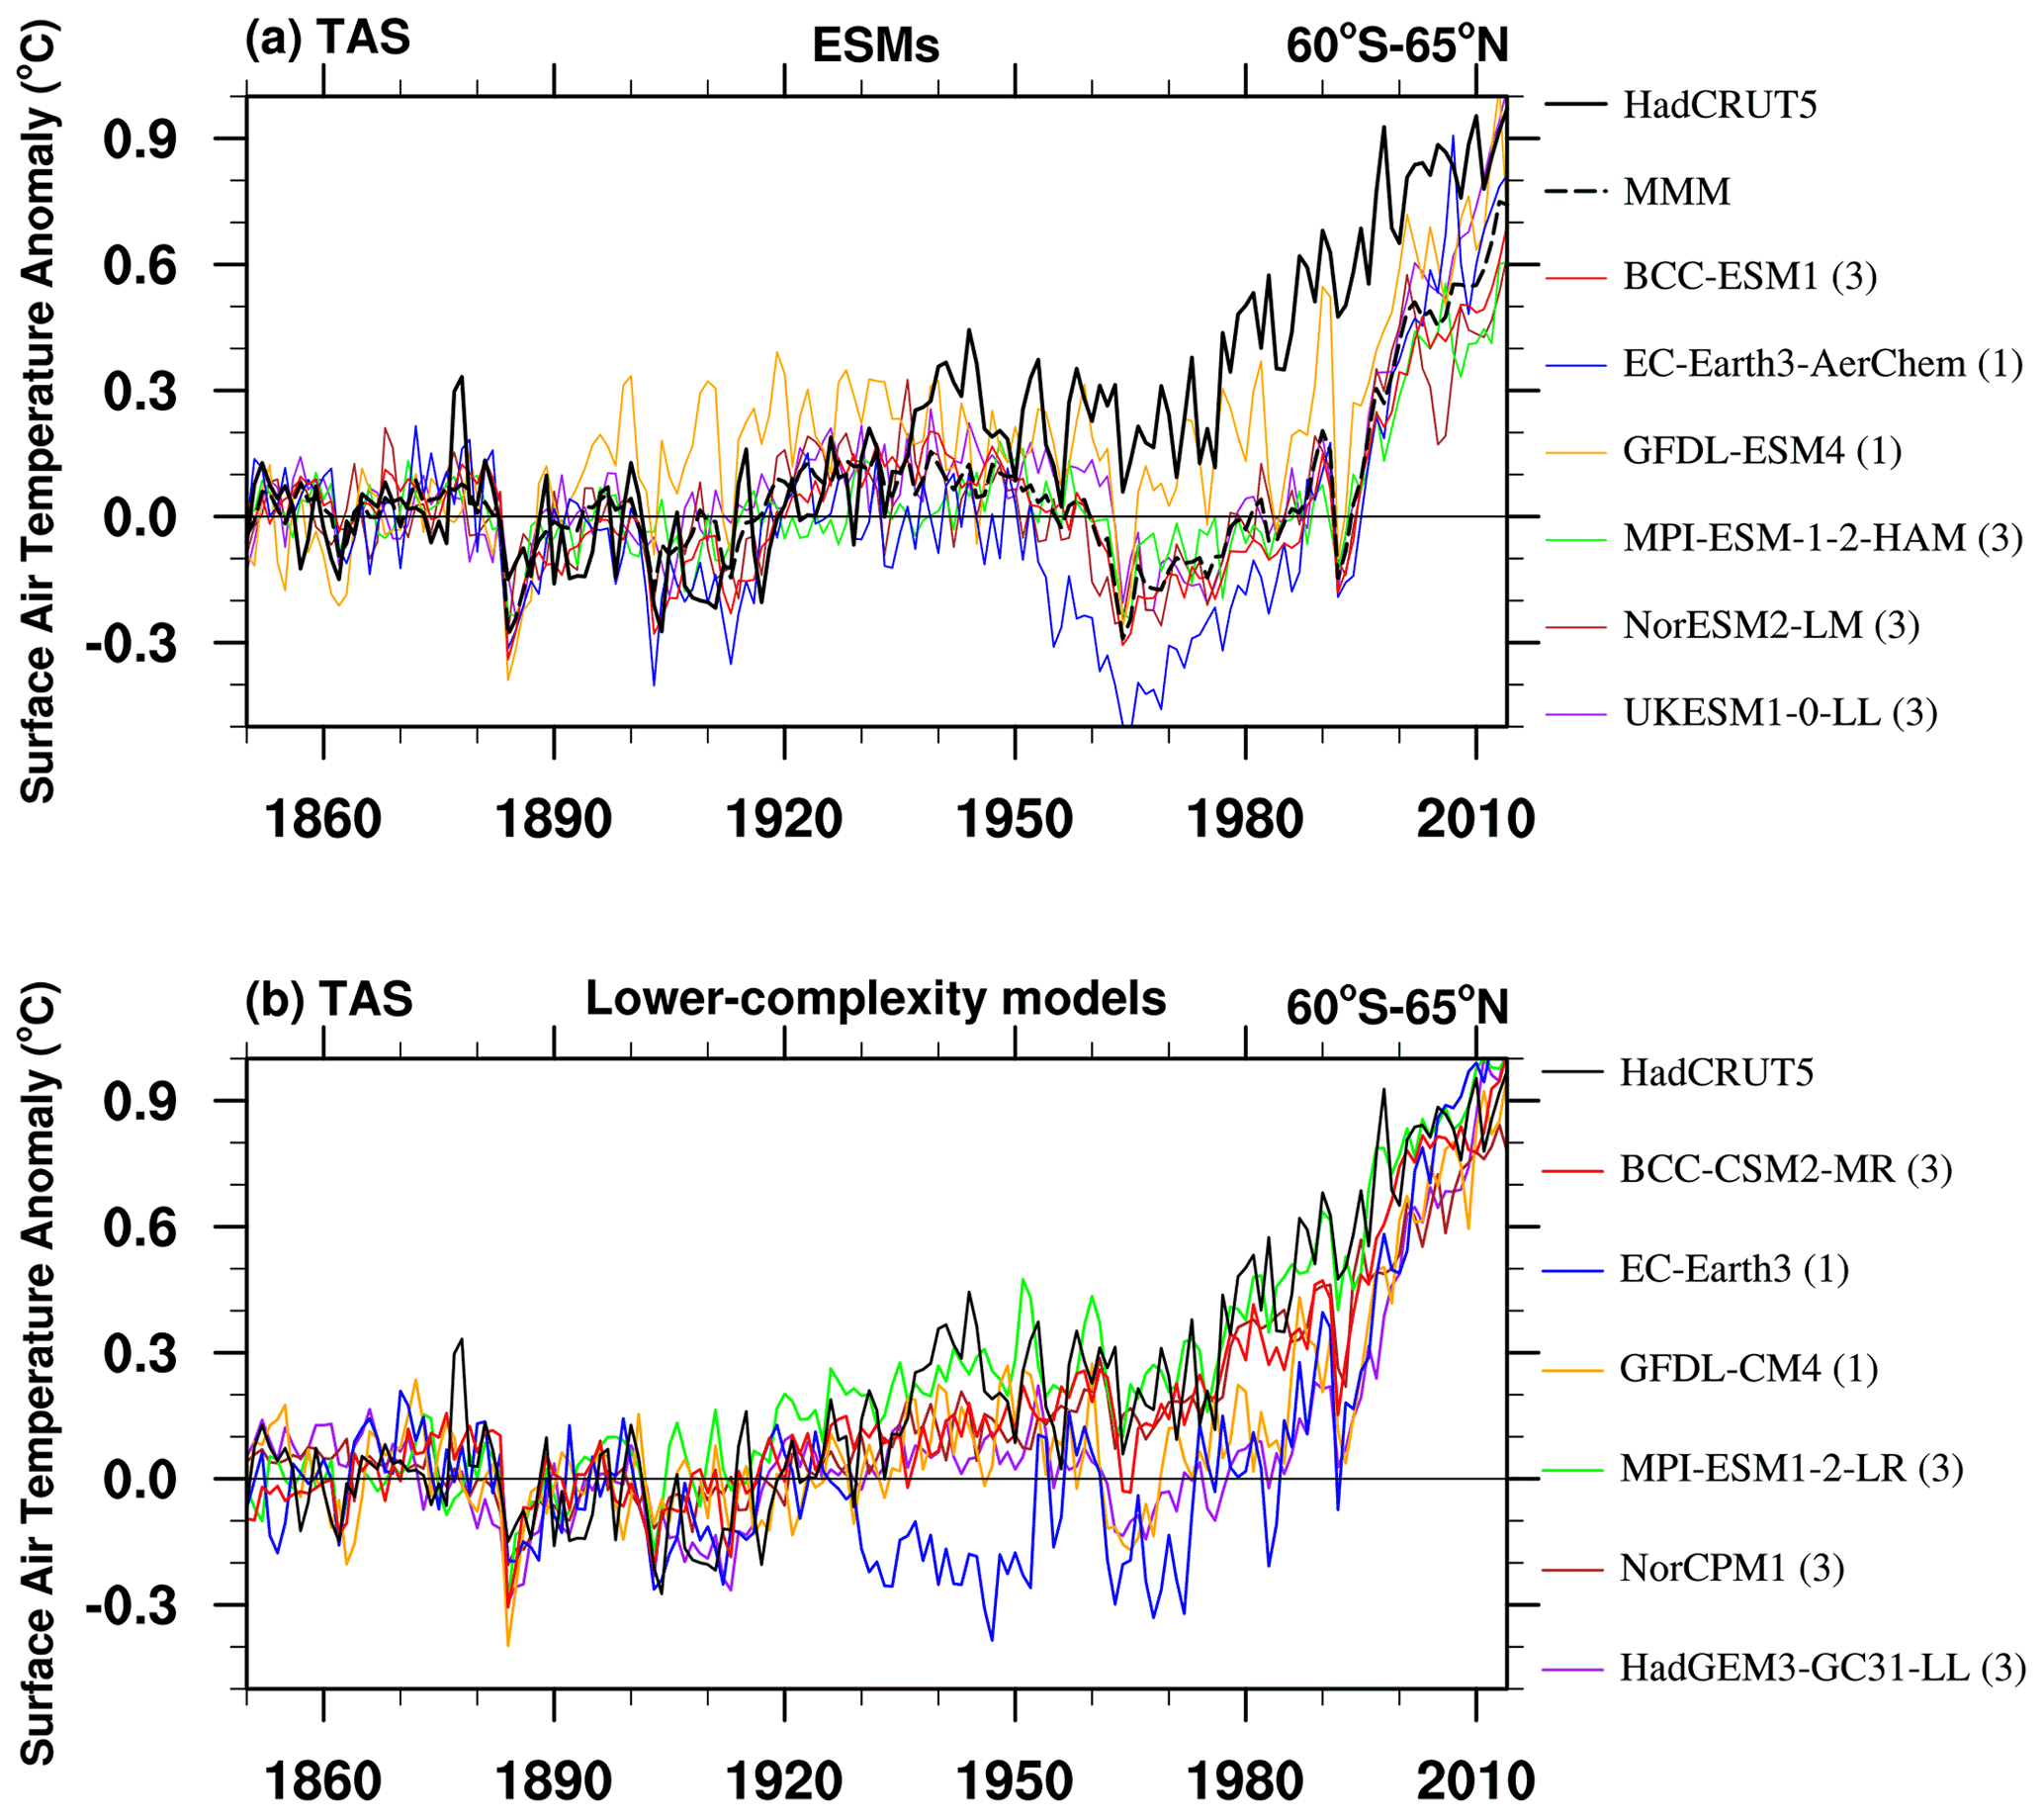
\includegraphics[width=6in]{Chapter1/figs/pothole_figure_Zhang2021.png}
    \caption[Anomalous cooling in the Earth system models participating in CMIP6]{(a) Historical near-global mean (60$^\circ$ S to 60$^\circ$ N) surface air temperature anomalies relative to 1850--1900 surface air temperature (TAS) from HadCRUT5 (thick black line), the ensemble mean for each ESM (solid colour lines), and multi-model mean (MMM, dashed black line). Panel (b) is the same as panel (a) but for the lower-complexity models. Units: $^\circ$C. Value in bracket is the number of available members for each model. \citep{zhangRoleAnthropogenicAerosols2021}.}
    \label{fig:zhang-pothole}
\end{figure}

In CMIP5, two separate configurations of the Met Office Unified Model were used. HadGEM3, being a coupled model with simplified, offline chemistry, participated in the historical simulations for CMIP5 climate projections,  while the UKCA chemistry-climate model, run in atmosphere-only mode but with online chemistry, took part in the Atmospheric Chemistry and Climate Model Intercomparison Project (ACCMIP) focusing on chemistry-climate interactions. The UKESM1 developed for CMIP6, brought online chemistry into a coupled atmosphere-ocean model, having been developed from the Met Office Unified Model and UKCA with the addition of Earth system modules.


The study by \citet{zhangRoleAnthropogenicAerosols2021} indicated that 6 models, table \ref{tab:zhang-model}, that participated in the CMIP6 tended to underestimate surface air temperature (TAS) during the period 1960--1990, known as the “pothole” period. This period coincided with elevated industrial activities over the Northern Hemisphere, especially in the Western European region. \ce{SO2} emitted by these industrial activities was one of the precursors of atmospheric sulfate aerosols which cooled down the atmosphere via aerosol direct and indirect effects. By comparing historical simulations with and without anthropogenic aerosol precursor emission, the study showed that anthropogenic emission led to more aerosol generation, with aerosol-cloud interaction accounting for up to 87\% of the aerosol forcing sensitivity. In addition, the study also indicated that the UKESM1 has the largest aerosol forcing sensitivity. 


\begin{small}
\begin{longtable}{>{\raggedright}p{3.25cm} >{\raggedright}p{3.25cm} >{\raggedright}p{3.5cm} >{\raggedright\arraybackslash}p{3.5cm}}
    \caption[Information of models included in the study by \citet{zhangRoleAnthropogenicAerosols2021}]{Information of models included in the study by \citet{zhangRoleAnthropogenicAerosols2021}}
    \label{tab:zhang-model}
    \\
    \toprule
     Model developer (Model) & Tropospheric chemistry model & Sulfur chemistry scheme & Aerosol scheme \\
     \midrule
     \endfirsthead

    \toprule
     Model developer (Model) & Tropospheric chemistry model & Sulfur chemistry scheme & Aerosol scheme \\
     \midrule
     \endhead
     
     \bottomrule
     \endlastfoot

     
     Met Office’s Hadley Centre for Climate Prediction and Research; MOHC (UKESM1-0-LL) Ref. \citet{sellarUKESM1DescriptionEvaluation2019,archibaldDescriptionEvaluationUKCA2020,mulcahyDescriptionEvaluationAerosol2020}  & UKCA (United Kingdom Chemistry and Aerosol) model with unified stratospheric-tropospheric chemistry (StratTrop) & Prognostic oxidant fields. Prognostic sulfur chemistry. & Aerosol scheme GLOMAP-mode. Two-moment, five size modes. 4 species: sulfate (\ce{SO4}), black carbon (BC), organic matter (OM) and sea salt. \\
     \midrule
     Norwegian Climate Center; NCC (NorESM2-LM). Ref. \citet{kirkevagProductiontaggedAerosolModule2018, selandOverviewNorwegianEarth2020} & Atmosphere model component CAM6-Nor built improvements on the CAM6 version from CESM2.1 & Diagnostic tropospheric oxidant fields: OH, \ce{O3}, \ce{H2O2}.  Prognostic  sulfur chemistry & 4 aerosol modes. 6 species: SOA, BC, \ce{SO4}, OM, Seasalt, and dust.  \\ 
     \midrule
     Max Planck Institute for Meteorology; MPI (MPI-ESM-1-2-HAM) Ref. \citet{neubauerGlobalAerosolClimate2019,neubauerHAMMOZConsortiumMPIESM12HAM2019,tegenGlobalAerosolClimate2019} & Atmospheric Model Component ECHAM6.3. &  Diagnostic oxidant fields: OH, \ce{H2O2}, \ce{NO2}, \ce{O3}, and \ce{NO3}. Prognostic sulfur chemistry. & Aerosol scheme HAM2.3. Two-moment. 7 modes: 4 soluble and 3 insoluble \\
     \midrule
     US Department of Commerce/ NOAA/Geophysical Fluid Dynamics Laboratory; GFDL (GFDL-ESM4) Ref. \citet{zhaoGFDLGlobalAtmosphere2018, heldStructurePerformanceGFDL2019, dunneGFDLEarthSystem2020} & Atmospheric component AM4.1 & Prognostic oxidant fields: OH, \ce{O3}, \ce{H2O2}, \ce{NO3}. Prognostic sulfur chemistry. & 5 aerosol types: sulfate, dust, black carbon, organic carbon, and sea salt.  \\
     \midrule
     European consortium of meteorological services, research institutes, and high-performance computing centers (EC-Earth-AerChem) Ref. \citet{vannoijeECEarth3AerChemGlobalClimate2021} & Aerosols and atmospheric chemistry are simulated with the Tracer Model version 5 (TM5), specifically release 3.0 of the massively parallel version of TM5 (TM5-mp 3.0). & The model includes aqueous-phase reactions for the oxidation of total dissolved sulfur dioxide & Modal aerosol microphysical scheme M7. 5 aerosol types: \ce{SO4}, BC, OA, sea salt, and mineral dust. 7 modes: 4 water-soluble and 3 insoluble modes  \\
     \midrule
     Beijing Climate Center; BCC (BCC-ESM1) Ref. \citet{zhangBCCESM1ModelDatasets2021} &  Atmospheric component is BCCAGCM3-Chem based on MOZART2 & Prognostic oxidant fields. Prognostic sulfur chemistry. & 5 aerosol species: \ce{SO4}, OC, BC, soil dust, and sea salt \\


\end{longtable}
\end{small}

One aspect of the historical experiment that remains of interest is the impact of emission migration equatorward and eastward in the last century and its implication and current state of understanding. Industrialization has led to rapid increases in greenhouse gas emissions along with aerosol precursors in many locations. The Industrial Revolution started in the Western European region with anthropogenic emissions peaking in 1980 followed by other regions such as the Indian subcontinent and Eastern Asia. It could be said that anthropogenic emissions have shifted eastwards and equatorward in the last 50 years.  \citet{zhangTroposphericOzoneChange2016} studied the effect of ozone precursor emission redistribution over the period 1980 to 2010 using climate models. The study separated the change in the magnitude of ozone precursor emission from the shift in emission location and concluded that the global tropospheric ozone change in this period is mainly due to the shift in the emission region rather than the magnitude of emission. Hence, the atmosphere is sensitive to emission location. Whether aerosol precursor emission migration which concurred with ozone precursor migration would lead to the same effect as ozone is not yet determined, and will be the focus of my work in the next six months.



\section{Aims and research questions}

Along with investigating the role of atmospheric chemistry in climate models, the overarching question of this work is to investigate the anomalous cooling period in the ESM by investigation of the \ce{SO2} oxidation pathways. Although \citet{zhangRoleAnthropogenicAerosols2021} identified the positive correlation between anomalous cooling and sulfate loading, the chemical and physical processes that lead to the overestimation of aerosol loading during the cooling period have not been identified. Identifying the processes and/or interactions within the climate model will improve future prediction capacity and reduce the uncertainty in aerosol forcing calculation. In addition, this project seeks to understand the effects of cloud droplets' pH on aerosol formation and radiative forcing and how pH affects model performance. 

In detail, this research aims to answer the following questions with respective aims and objectives.

\begin{enumerate}
    \item  How do \ce{SO2} budget and oxidation tendencies respond to changes in oxidant levels over the historical period?
    \begin{itemize}
        \item To understand the sulfate formation processes, the first part of this project focuses on sulfate chemistry in UKESM1 over the historical period. This work aims to utilise the data available from the CMIP6 and its endorsed project such as the AerChemMIP to study sulfate aerosols formation.  
        \item Sulfate production involves \ce{SO2} reaction with other precursors such as \ce{O3}, OH, and \ce{H2O2}. This part explores the global trends of sulfur budget and oxidation tendencies. It takes AerChemMIP transient experiments that perturb the oxidant levels such as \textit{histSST}, \textit{histSST-piO3}, etc., and investigates model sensitivity to oxidant changes. 
    \end{itemize}

    \item How does sulfate aerosol size distribution respond to oxidant perturbation?

    \begin{itemize}
        \item Oxidant level changes will have a knock-on effect on aerosol formation since \ce{SO2} oxidation forms aerosol and this process depends on the oxidant availability. The transient historical prescribed SST simulations from the AerChemMIP are useful for studying the attribution of climatic changes to precursor emissions. This section aims to quantify aerosol size distribution changes caused by oxidant level changes by comparing transient historical prescribed SST simulations experiments with the controlled \textit{histSST} experiment. 
    \end{itemize}

    \item At the process level, how do oxidant changes affect aerosol radiative forcing due to changes in oxidants?

    \begin{itemize}
        \item Aerosol radiative forcing is an important climate forcing with the largest uncertainty in the IPCC AR6 assessment. Building on our understanding of the underpinning aerosol production channels and sulfate burden, this part explores the climatic responses due to oxidant changes. 
    \end{itemize}

    \item How do changes in seasonal levels of oxidants affect aerosol formation and subsequent radiative effects?

    \begin{itemize}
        \item There are observed seasonal trends in oxidants from measurement and modelling studies.
        \item The UKESM1 can simulate both aerosol mass and number independently, making it one of the most robust climate models regarding aerosol simulation. GLOMAP-mode which is the aerosol module used in UKESM1 simulates both soluble and insoluble aerosols in four modes: nucleation, Aitken, accumulation and coarse and different aerosol types: sulfate, sea salt, organic, dust and black carbon. It also simulates interaction between modes such as coagulation and condensation as well as wet and dry deposition. This makes the UKESM1 a useful tool for studying the aerosol properties in different seasons.
    \end{itemize}

    \item The emission of aerosol precursors shifted eastwards and equatorward away from the European region since 1980. What is the effect of emission location change on oxidation tendencies?

    \begin{itemize}
        \item This part of the project explores regional sulfate formation and regional differences due to chemical background. In the historical period, anthropogenic emissions, including \ce{SO2}, increased with industrial activities in the European region and peaked in 1980 before decreasing. Then, emissions increased in Eastern Asia and reached their peak in the 200s. Since \ce{SO2} emission location dictates the background of available precursors and the atmospheric chemistry condition near the equator differs from that of the extratropical region, it is possible that different regions have different baseline oxidation tendencies and also behave differently to oxidant level changes. This section builds on Research Question 1 and further inspects the details in regions, aiming to find out the characteristics of oxidation in different time periods and regions.  
    \end{itemize}

    \item How does discrepancy in oxidant field affect aerosol formation and subsequent radiative effects?

    \begin{itemize}
        \item  We have access to an offline oxidant version of UKESM1, prepared by Alistair Sellar at UK Met Office, and to the data from the first sensitivity histSST experiments in which UKESM1 oxidants were replaced by those from analogous CESM2 experiments.  I plan to investigate the sulfur budget in these experiments, and to quantify the differences in both oxidant field and oxidant chemistry to determine the sensitivity of the aerosol chemistry to the oxidant fields in a way that complements the approach taken in Chapter 3 where \textit{histSST-piO3} and other experiments were analysed. To connect oxidant changes to ERF, we would need to set up other timeslice experiments. This work could be extended to investigate aspects of the radiative forcing such as the role of oxidant in ERFaci and other climate diagnostics. 
    \end{itemize}
    
\end{enumerate}

\section{Thesis structure and publication work}

Firstly, this thesis describes the work in preparation for publication which quantifies the role of SLCFs including methane and ozone precursors in modifying radiative balance through changes in aerosol formation (Chapter \ref{ch3}). Secondly, I describe how the seasonal cycle modifies SO2 oxidation and changes the radiative effects. Thirdly, oxidation is explored in the view of regional changes and its contribution to regional cooling. Finally, the sensitivity of SO2 oxidation to oxidants is explored in the final chapter.